\documentclass[11pt,a4paper]{article}
\usepackage[utf8]{inputenc}
\usepackage[T1]{fontenc}
\usepackage[brazilian]{babel}
\usepackage{graphicx,booktabs,float}
\usepackage[a4paper,margin=2.5cm]{geometry}
\usepackage[hidelinks]{hyperref}
\title{O CVSS é um bom critério para priorizar a correção de vulnerabilidades? Evidências da NVD e do catálogo KEV da CISA (2021–2025)}
\author{Daniel de Carvalho Vianna\\ Departamento de Engenharia de Produção, Universidade de Brasília (UnB)}
\date{09/11/2026}
\begin{document}
\maketitle

\begin{abstract}
Este trabalho avalia se priorizar a correção de vulnerabilidades apenas pela severidade CVSS é eficiente, comparando as CVEs publicadas entre 01/01/2021 e 31/12/2025 na National Vulnerability Database (NVD) com o catálogo de vulnerabilidades exploradas (KEV) da CISA. Das 162.141 CVEs analisadas, 870 constam no KEV; as faixas crítica e alta contêm 87,4\% das CVEs do KEV, mas apenas 0,92\% das CVEs críticas/altas foram exploradas. Segundo o critério declarado, a hipótese de ineficiência é CONFIRMADA.
\end{abstract}

\section{Introdução}
Equipes de TI recebem milhares de vulnerabilidades por ano e têm capacidade de correção limitada, um problema de alocação de recursos escassos sob risco. A prática usual é corrigir primeiro as vulnerabilidades críticas e altas segundo o CVSS \cite{cvss}. Este trabalho testa a hipótese de que priorizar apenas pelo CVSS gera um backlog grande e pouco eficiente, usando a exploração real registrada no catálogo KEV \cite{kev} como referência. Estudos anteriores já apontam diferenças entre severidade e exploração \cite{allodi,epss}.

\section{Método}
\subsection{Dados e coleta}
Foram coletadas, pela API 2.0 da NVD \cite{nvd} sem chave de acesso, as CVEs publicadas entre 01/01/2021 e 31/12/2025, em janelas de até 120 dias, com 500 CVEs por página, retentativas com espera exponencial e retomada. Foram obtidas 170.006 CVEs (838,5 MB em JSON) entre 2026-11-09 11:38:54 e 2026-11-09 12:26:30 (UTC), conferidas janela a janela contra o total anunciado pela API. O catálogo KEV \cite{kev} foi obtido em CSV (1.769 linhas). O recorte começa em 2021 porque o KEV só existe desde novembro de 2021. Os dados são públicos e não contêm dados pessoais.

\subsection{Pipeline e regras de negócio}
O pipeline foi executado em um notebook do Google Colab, com ETL em PySpark local (arquitetura medalhão: raw, bronze, silver, gold) e persistência das camadas silver e gold no BigQuery Sandbox, com conferência das contagens de linhas. O modelo gold é uma estrela com a tabela fato fato\_cve (grão: uma CVE) e as tabelas dim\_data, dim\_cwe e ponte\_cve\_vendor. Regras: CVSS v3.1, senão v3.0, senão SEM\_CVSS; primeiro CWE listado; vendor extraído do CPE 2.3 apenas de configurações vulneráveis; junção NVD-KEV por cve\_id em maiúsculas; deduplicação por maior lastModified; exclusão de CVEs rejeitadas; janelas negativas excluídas de P4.

\subsection{Critério de avaliação da hipótese}
Definiu-se, antes da execução, a precisão (percentual das CVEs críticas e altas presentes no KEV) e a cobertura (percentual das CVEs do KEV contidas nas faixas crítica e alta). A hipótese é confirmada se a precisão for inferior a 10\% e a cobertura inferior a 90\%; parcialmente confirmada se apenas um critério for atendido; refutada se nenhum for.

\section{Resultados}
\subsection{Evolução anual (P1)}
O volume anual de CVEs (excluídas as 7.865 rejeitadas) foi de 20.149 em 2021 e de 48.150 em 2025, uma alta de 139,0\%; o maior volume ocorreu em 2025 (48.150 CVEs). Entre as CVEs que possuem CVSS v3.x, as críticas e altas representaram 55,7\% em 2021 e 49,2\% em 2025, 52,1\% no conjunto do período — parcela expressiva (40\% ou mais). No total, a fila prioritária por CVSS (críticas + altas) soma 82.854 CVEs em 5 anos (média de 16.571 por ano, ou cerca de 45,4 por dia).
\begin{figure}[ht]
\centering
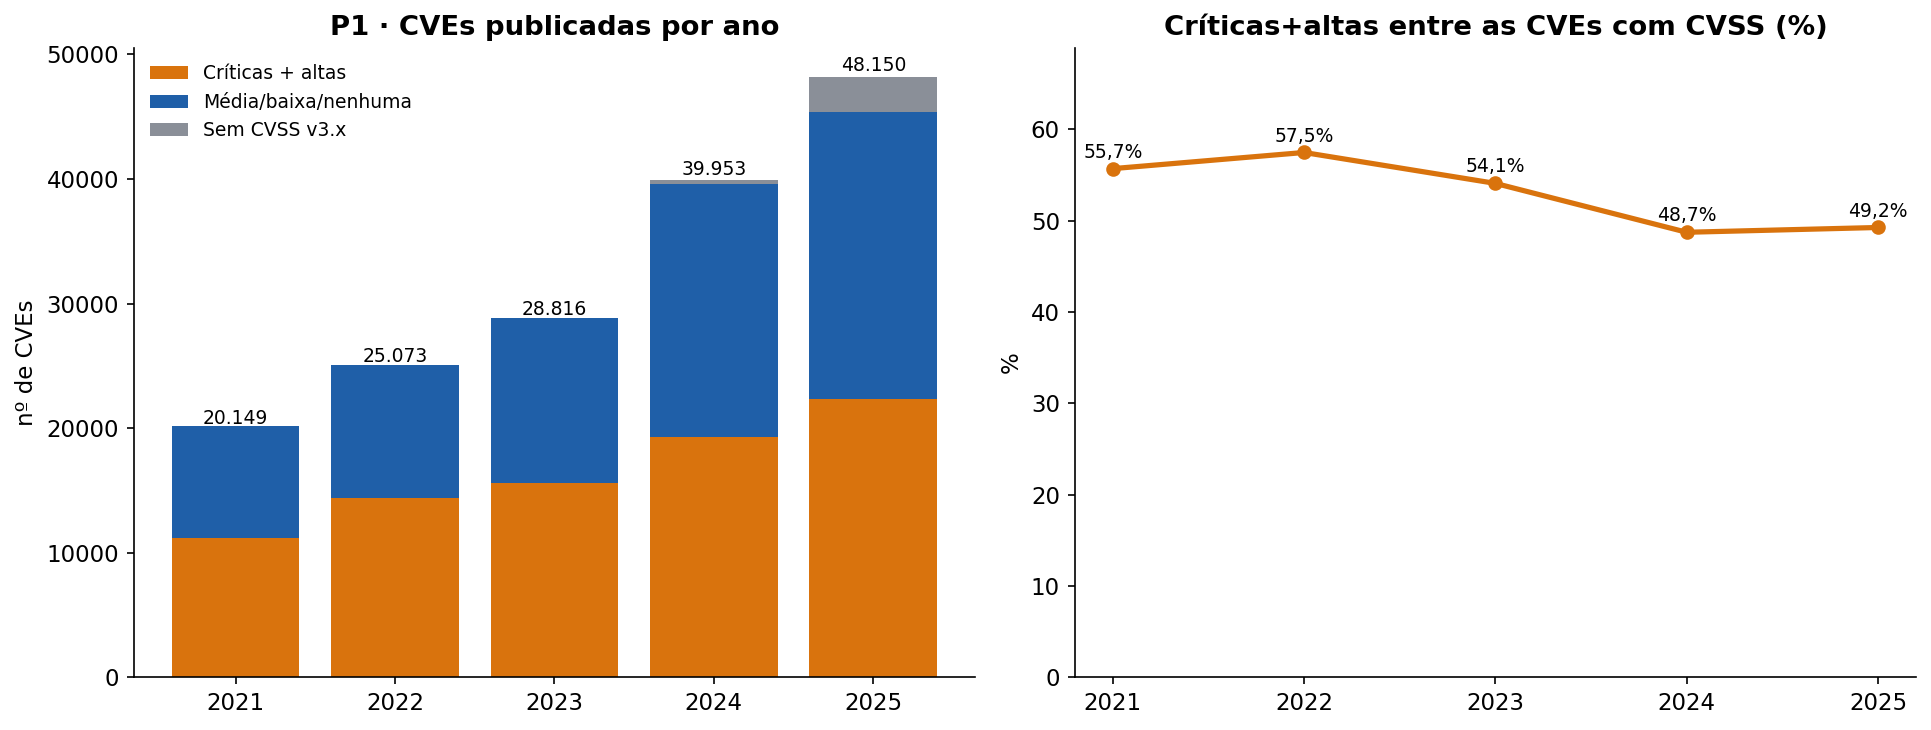
\includegraphics[width=\linewidth]{p1.png}
\caption{Volume anual de CVEs e participação de críticas/altas.}
\label{fig:p1}
\end{figure}
\subsection{CWEs das CVEs críticas (P2)}
Há 22.566 CVEs críticas (CVSS $\geq$ 9) no período. As três CWEs específicas mais frequentes entre elas são: CWE-89 (Injeção de SQL) com 3.915 CVEs (17,3\%); CWE-74 (Injeção) com 1.883 CVEs (8,3\%); CWE-787 (Escrita fora dos limites) com 1.162 CVEs (5,1\%). As cinco principais CWEs específicas concentram 40,0\% das críticas. Outras 1.456 CVEs críticas (6,5\%) estão classificadas em categorias genéricas da NVD (NVD-CWE-Other/noinfo) ou sem CWE, o que limita a orientação de treinamento por tipo de falha.
\begin{figure}[ht]
\centering
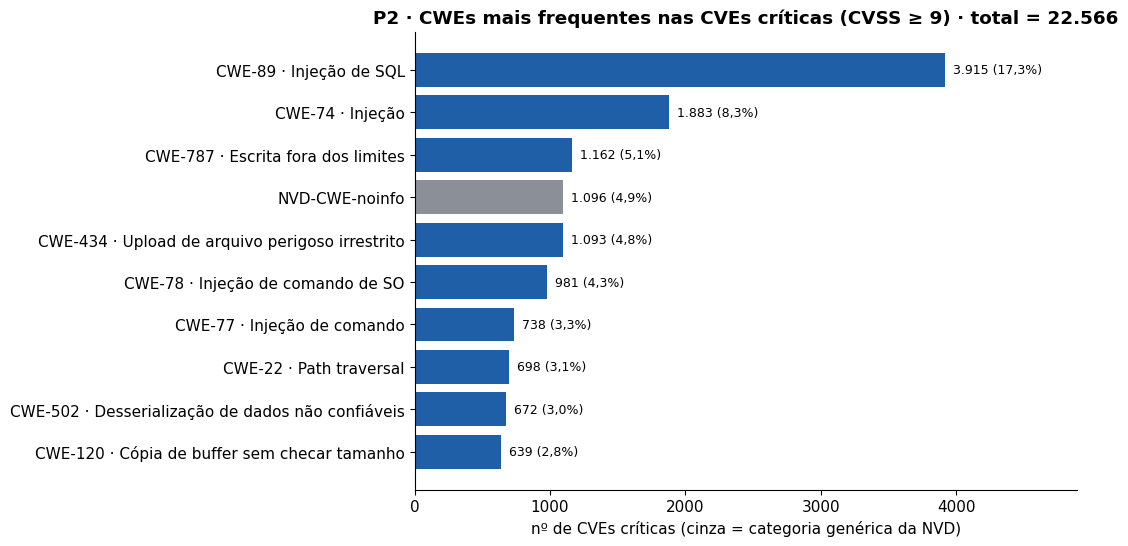
\includegraphics[width=\linewidth]{p2.png}
\caption{CWEs mais frequentes entre as CVEs críticas.}
\label{fig:p2}
\end{figure}
\subsection{Exploração por faixa de severidade (P3)}
Das 162.141 CVEs do recorte, 870 constam no KEV (0,54\%). A taxa de exploração por faixa foi: crítica 1,39\% (314 de 22.566), alta 0,74\% (446 de 60.288), média 0,15\% (107 de 72.901), baixa 0,09\% (3 de 3.282) e sem CVSS v3.x 0,00\% (0 de 3.102). A taxa decresce da faixa crítica para a baixa. A taxa das críticas é 9,5 vezes a das médias. Priorizar críticas e altas implica corrigir 82.854 CVEs para alcançar 760 exploradas: precisão de 0,92\% (aproximadamente 109 CVEs críticas/altas corrigidas para cada uma que consta no KEV; 1,7 vez a taxa média do universo). Quanto à cobertura, as faixas crítica e alta contêm 760 das 870 CVEs do KEV (87,4\%); 110 CVEs exploradas (12,6\%) ficam fora da fila crítica/alta, das quais 0 não têm CVSS v3.x.
\begin{table}[ht]
\centering\small
\begin{tabular}{lrrrr}
\toprule
Faixa & CVEs & No KEV & \% exploradas & \% do KEV \\
\midrule
Crítica & 22.566 & 314 & 1,39\% & 36,1\% \\
Alta & 60.288 & 446 & 0,74\% & 51,3\% \\
Média & 72.901 & 107 & 0,15\% & 12,3\% \\
Baixa & 3.282 & 3 & 0,09\% & 0,3\% \\
Nenhuma (0,0) & 2 & 0 & 0,00\% & 0,0\% \\
Sem CVSS v3.x & 3.102 & 0 & 0,00\% & 0,0\% \\
\bottomrule
\end{tabular}
\caption{Exploração (KEV) por faixa de severidade CVSS.}
\label{tab:p3}
\end{table}
\begin{figure}[ht]
\centering
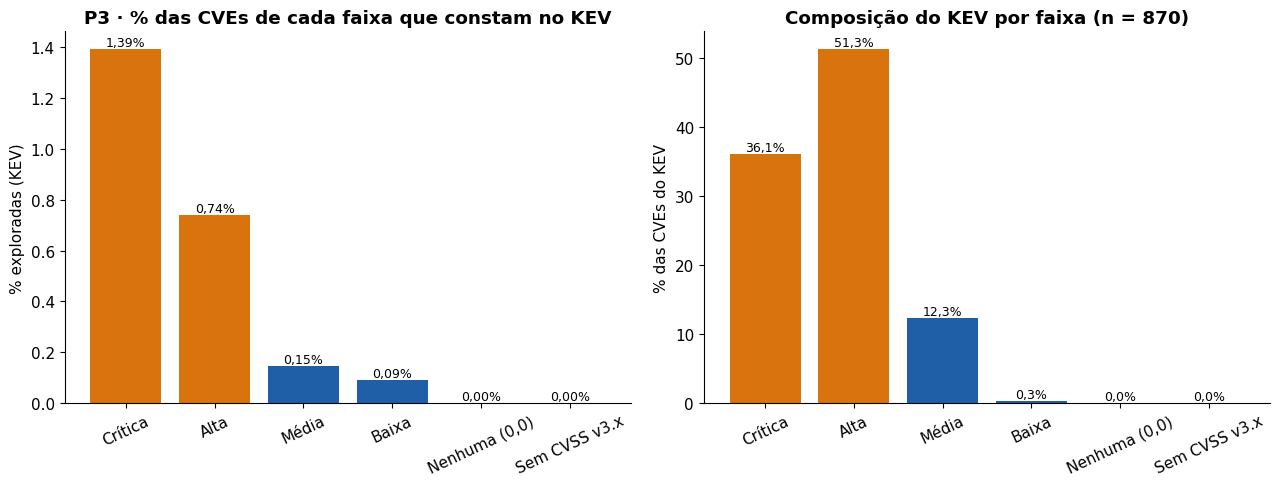
\includegraphics[width=\linewidth]{p3.png}
\caption{Taxa de exploração por faixa de severidade e composição do KEV.}
\label{fig:p3}
\end{figure}
\subsection{Janela publicação $\rightarrow$ KEV (P4)}
Considerando 808 CVEs do KEV com janela não negativa, a mediana entre a publicação na NVD e a inclusão no KEV foi de 49 dias e o p90 de 569 dias; 43,6\% entraram no KEV em até 30 dias. Por ano de publicação, a mediana foi de 208 dias em 2021 e 10 em 2025. Foram excluídas 62 CVEs com janela negativa (incluídas no KEV antes de publicadas na NVD). A cauda é longa (p90 acima de um ano): parte relevante das CVEs só é reconhecida como explorada muito depois da publicação, de modo que um prazo (SLA) curto e único não captura esses casos e o monitoramento do KEV precisa ser contínuo. Cautela: há censura à direita — CVEs publicadas em anos mais recentes tiveram menos tempo de observação até a data da coleta (2026-11-09), o que tende a reduzir mediana e p90 desses anos.
\begin{table}[ht]
\centering\small
\begin{tabular}{lrrrr}
\toprule
Ano & n & Mediana (dias) & p90 (dias) & \% até 30 dias \\
\midrule
2021 & 212 & 208 & 1.070 & 7,1\% \\
2022 & 99 & 69 & 818 & 36,4\% \\
2023 & 153 & 8 & 617 & 61,4\% \\
2024 & 154 & 18 & 307 & 57,1\% \\
2025 & 190 & 10 & 210 & 62,6\% \\
\bottomrule
\end{tabular}
\caption{Janela entre publicação e inclusão no KEV, por ano de publicação.}
\label{tab:p4}
\end{table}
\begin{figure}[ht]
\centering
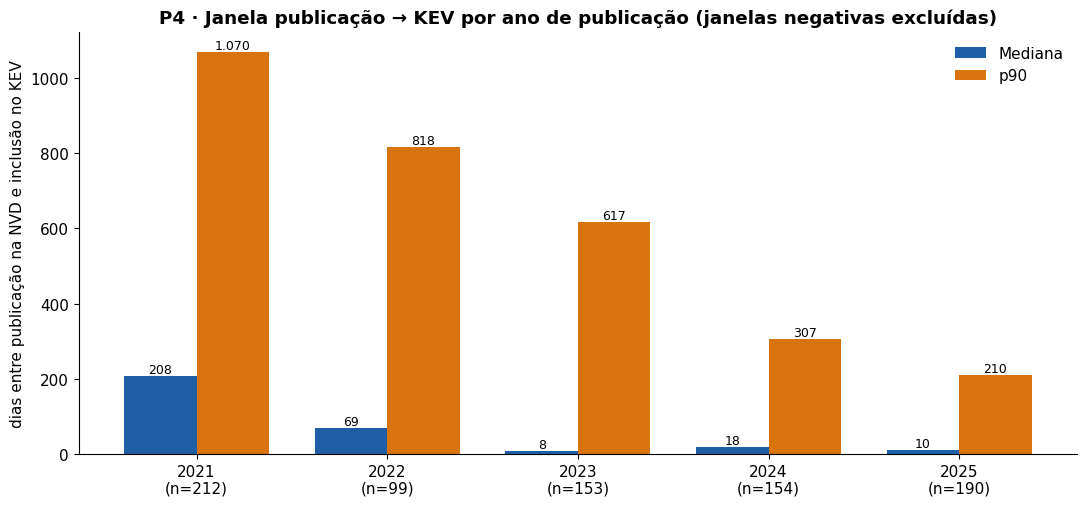
\includegraphics[width=\linewidth]{p4.png}
\caption{Mediana e p90 da janela entre publicação e inclusão no KEV.}
\label{fig:p4}
\end{figure}
\subsection{Fabricantes com CVEs exploradas (P5)}
Pelo vendor extraído do CPE (apenas configurações marcadas como vulneráveis), os fabricantes com mais CVEs no KEV são: microsoft (174); apple (79); debian (69); google (68); fedoraproject (66). Cobertura do mapeamento: 100,0\% das 870 CVEs do KEV possuem vendor. Uma CVE pode ter vários vendors (por exemplo, o fabricante do produto e as distribuições que o empacotam, como debian e fedoraproject), logo as contagens por vendor se sobrepõem e não devem ser somadas. Verificação cruzada com o campo vendorProject do próprio KEV: Microsoft (163); Apple (72); Google (53); Cisco (25); Ivanti (25).
\begin{figure}[ht]
\centering
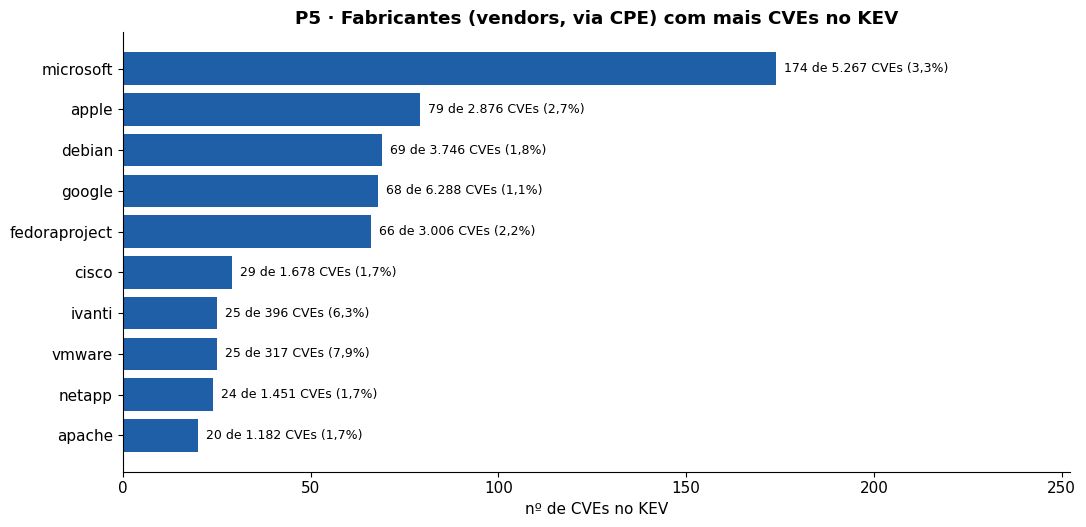
\includegraphics[width=\linewidth]{p5.png}
\caption{Fabricantes com mais CVEs no KEV.}
\label{fig:p5}
\end{figure}

\section{Discussão}
Critério declarado antes da execução: a hipótese é CONFIRMADA se (C1) a precisão das faixas crítica+alta for inferior a 10\% e (C2) a cobertura do KEV por essas faixas for inferior a 90\%; PARCIALMENTE CONFIRMADA se apenas um dos dois critérios for atendido; REFUTADA se nenhum for. Resultado: precisão = 0,92\% (C1 atendido) e cobertura = 87,4\% (C2 atendido). Veredito: hipótese CONFIRMADA. A leitura literal da hipótese (a maioria das críticas/altas nunca é explorada) é satisfeita, pois 99,08\% das CVEs críticas/altas não constam no KEV. Implicação: usar apenas o CVSS como critério de priorização gera uma fila grande e de baixo rendimento e, ao mesmo tempo, deixa de fora uma parcela relevante das CVEs efetivamente exploradas. Uma política mais eficiente combina o CVSS com um sinal de exploração: tratar primeiro as CVEs presentes no KEV (e, em extensão futura, com alta probabilidade pelo EPSS) e usar o CVSS para ordenar o restante. Ressalvas: o KEV registra apenas exploração conhecida e relevante para o governo dos EUA (subnotificação), e os critérios numéricos (10\% e 90\%) são uma escolha do autor, explicitada para que o resultado seja auditável; outros limiares podem alterar o veredito.

\section{Qualidade dos dados e limitações}
A análise de qualidade cobriu completude, unicidade, conformidade, consistência, acurácia e atualidade; os resultados detalhados estão no repositório (README e figuras de qualidade).
\begin{itemize}
\item O KEV registra apenas exploração conhecida (subnotificação) e tem viés para produtos relevantes ao governo dos EUA.
\item 1,9\% das CVEs analisadas (3.102 de 162.141) não possuem CVSS v3.x (CVSS v4.0 não foi considerado).
\item 19,8\% das CVEs da camada silver (incluindo as rejeitadas) não têm vendor mapeado via CPE.
\item Censura à direita: CVEs de 2025 tiveram pouco tempo para entrar no KEV até a coleta (2026-11-09).
\item Os limiares do critério de veredito (10\% e 90\%) são uma escolha do autor.
\end{itemize}

\section{Conclusão}
Nos dados de 2021–2025, a hipótese de que o CVSS isolado é pouco eficiente como critério de priorização é CONFIRMADA, segundo o critério declarado. Como trabalhos futuros, sugerem-se a inclusão do EPSS \cite{epss}, do CVSS v4.0 e uma coleta incremental contínua.

\begin{thebibliography}{9}
\bibitem{nvd} NIST. \textit{National Vulnerability Database -- CVE API 2.0}. \url{https://nvd.nist.gov/developers/vulnerabilities}.
\bibitem{kev} CISA. \textit{Known Exploited Vulnerabilities Catalog}. \url{https://www.cisa.gov/known-exploited-vulnerabilities-catalog}.
\bibitem{cvss} FIRST. \textit{Common Vulnerability Scoring System v3.1: Specification Document}. \url{https://www.first.org/cvss/v3.1/specification-document}.
\bibitem{epss} Jacobs, J.; Romanosky, S.; Edwards, B.; Adjerid, I.; Roytman, M. Exploit Prediction Scoring System (EPSS). \textit{Digital Threats: Research and Practice}, 2(3), 2021.
\bibitem{allodi} Allodi, L.; Massacci, F. Comparing vulnerability severity and exploits using case-control studies. \textit{ACM Transactions on Information and System Security}, 17(1), 2014.
\end{thebibliography}
\end{document}
